%%%%%%%%%%%%%%%%%%%%%%%%%%%%%%%%%%%%%%%%%
% baposter Landscape Poster
% LaTeX Template
% Version 1.0 (11/06/13)
%
% baposter Class Created by:
% Brian Amberg (baposter@brian-amberg.de)
%
% This template has been downloaded from:
% http://www.LaTeXTemplates.com
%
% License:
% CC BY-NC-SA 3.0 (http://creativecommons.org/licenses/by-nc-sa/3.0/)
%
%%%%%%%%%%%%%%%%%%%%%%%%%%%%%%%%%%%%%%%%%

%----------------------------------------------------------------------------------------
%	PACKAGES AND OTHER DOCUMENT CONFIGURATIONS
%----------------------------------------------------------------------------------------

\documentclass[landscape,a0paper,fontscale=0.285]{baposter} % Adjust the font scale/size here

\usepackage{graphicx} % Required for including images
\graphicspath{{figures/}} % Directory in which figures are stored

\usepackage{amsmath} % For typesetting math
\usepackage{amssymb} % Adds new symbols to be used in math mode

\usepackage{booktabs} % Top and bottom rules for tables
\usepackage{enumitem} % Used to reduce itemize/enumerate spacing
\usepackage{palatino} % Use the Palatino font
\usepackage[font=small,labelfont=bf]{caption} % Required for specifying captions to tables and figures

\usepackage{multicol} % Required for multiple columns
\setlength{\columnsep}{1.5em} % Slightly increase the space between columns
\setlength{\columnseprule}{0mm} % No horizontal rule between columns

\usepackage{tikz} % Required for flow chart
\usetikzlibrary{shapes,arrows} % Tikz libraries required for the flow chart in the template

\newcommand{\compresslist}{ % Define a command to reduce spacing within itemize/enumerate environments, this is used right after \begin{itemize} or \begin{enumerate}
\setlength{\itemsep}{1pt}
\setlength{\parskip}{0pt}
\setlength{\parsep}{0pt}
}


\newcommand{\bfSigma}{\mbox{\boldmath$\Sigma$}}
\newcommand{\bfLambda}{\mbox{\boldmath$\Lambda$}}


\DeclareMathOperator*{\argmax}{\arg\!\max}

\definecolor{lightblue}{rgb}{0.145,0.6666,1} % Defines the color used for content box headers

\begin{document}

\begin{poster}
{
headerborder=closed, % Adds a border around the header of content boxes
colspacing=1em, % Column spacing
bgColorOne=white, % Background color for the gradient on the left side of the poster
bgColorTwo=white, % Background color for the gradient on the right side of the poster
borderColor=lightblue, % Border color
headerColorOne=black, % Background color for the header in the content boxes (left side)
headerColorTwo=lightblue, % Background color for the header in the content boxes (right side)
headerFontColor=white, % Text color for the header text in the content boxes
boxColorOne=white, % Background color of the content boxes
textborder=roundedleft, % Format of the border around content boxes, can be: none, bars, coils, triangles, rectangle, rounded, roundedsmall, roundedright or faded
eyecatcher=true, % Set to false for ignoring the left logo in the title and move the title left
headerheight=0.1\textheight, % Height of the header
headershape=roundedright, % Specify the rounded corner in the content box headers, can be: rectangle, small-rounded, roundedright, roundedleft or rounded
headerfont=\Large\bf\textsc, % Large, bold and sans serif font in the headers of content boxes
%textfont={\setlength{\parindent}{1.5em}}, % Uncomment for paragraph indentation
linewidth=2pt % Width of the border lines around content boxes
}
%----------------------------------------------------------------------------------------
%	TITLE SECTION 
%----------------------------------------------------------------------------------------
%
{
\includegraphics[height=3em]{milalogo}} % First university/lab logo on the left
{\bf\textsc{Applying LSTM to text generation}\vspace{0.5em}} % Poster title
{\textsc{J. Leroux, N. Laliberte, S. Frederic Boileau \hspace{5pt}\hspace{5pt} }} % Author names and institution
{
\includegraphics[height=3em]{udemlogo}} % Second university/lab logo on the right

%----------------------------------------------------------------------------------------
%	INTRODUCTION
%----------------------------------------------------------------------------------------

\headerbox{Introduction}{name=introduction,column=0,row=0}{


\begin{itemize}\compresslist
\item A conditional independence graph is a concise representation of pairwise conditional independence among many variables.
\item We present a general framework for estimating pairwise conditional independence relationships among variables.
\end{itemize}
% When there are two boxes, some whitespace may need to be added if the one on the right has more content
}

%----------------------------------------------------------------------------------------
%	STABILITY SELECTION
%----------------------------------------------------------------------------------------

\headerbox{\small{Stability Selection Algorithm}}{name=stability,column=0,below=introduction,above=bottom}{

\begin{itemize}
	\item Number of edges is a tuning parameter in any graphical model estimator.
	\item No obvious number constitutes a good choice.
	\item Stability Selection helps choosing the \\ parameter $(\lambda)$ with respect to a bound on the expected number of false positives $\mu$ :
\end{itemize}
\begin{center}
	$ \lambda = \lfloor  \sqrt{ ( 2 \omega -1) \cdot \mu \cdot p \cdot (p-1)/2} \rfloor$
\end{center}
where $\omega$ is a threshold of the minimum relative frequency of edges and $p$ is the number of variables.

\tikzstyle{decision} = [diamond, draw, fill=blue!20, text width=4.5em, text badly centered, node distance=2cm, inner sep=0pt]
\tikzstyle{block} = [rectangle, draw, fill=blue!25, text width=20em, text centered, rounded corners, minimum height=3em]
\tikzstyle{block2} = [rectangle, draw, fill=blue!25, text width=15em, text centered, rounded corners, minimum height=4em]
\tikzstyle{block3} = [rectangle, draw, fill=blue!25, text width=10em, text centered, rounded corners, minimum height=4em]
\tikzstyle{line} = [draw, -latex']
\tikzstyle{cloud} = [draw, rectangle, fill=red!20, node distance=3.2cm, text width=6em, text centered, rounded corners, minimum height=2em]

\vspace{-.25 cm}
\begin{center}
	\textbf{Pseudo code}
\end{center}
\vspace{-.65 cm}

\begin{center}
\begin{tikzpicture}[node distance = 2cm, auto]
\node [block] (init) {Hyperparameters' initialization: 
	 $\omega$, $\mu$};
%\node [cloud, right of=init] (Start2) {Start Two};
\node [block3, below of=init] (bound) {Edges upper bound calculation ($\lambda$) given $\omega$ and $\mu$};
\node [block2, below of=bound] (learning) {Graph structure estimation with the learning procedure and $\lambda$};
\node [block2, below of=learning] (freq) {Calculation of the edges \\ frequency over the k graph};
\node [block, below of=freq] (final) {Estimation of the final graph structure in respect to the minimal frequency $\omega$};

\node [cloud, right of=bound] (boot) {k bootstraps resampling};
\path [line, dashed] (boot) |- (learning);
%\path (bound)   -- coordinate[midway] (m) (learning);
%\path [->] (boot.west) -- (m); 


\path [line] (init) -- (bound);
\path [line] (bound) -- (learning);
\path [line] (learning) -- (freq);
\path [line] (freq) -- (final);

%\path [line, dashed] (Start2) -- (init);
%\path [line, dashed] (Start2) |- (init2);
\end{tikzpicture}
\end{center}

\vspace{0 em} % When there are two boxes, some whitespace may need to be added if the one on the right has more content

}


%----------------------------------------------------------------------------------------
%	LEARNING PROCEDURES 
%----------------------------------------------------------------------------------------

\headerbox{Algorithms}{name=method,column=1,row=0}{

\vspace{0.2 cm}
\subsection*{Graphical Random Forest (GRaFo)}
Edges ranking scheme based on Random Forests' permutation importance measure.\\

\textbf{Importance measure} :\\  \\
Predictor's relevance based on error difference between a regular Random Forest fit and a Random Forest fit within which one predictor's values are permuted.\\

\textbf{Main steps} : 
\begin{enumerate}\compresslist
\item Perform RF regression of a single variable on the remaining $p-1$ variables.
\item Calculate predictors' importance measure.
\item Repeat steps 1 and 2 for every $p$ variables.
\item Define the $(i,j) $ pair as $i$ the outcome and $j$ the predictor.
\item Best $\lambda$ ranking pairs are added as edges.
\end{enumerate}


\vspace{0 cm}
\subsection*{Graphical Lasso (GLasso)}

Estimation of the regularized precision matrix $\bfLambda$  under multivariate normal hypothesis:

\begin{center}
	$\hat{\bfLambda}_{\text{GL}} = \argmax_{\bfLambda} \left\{ \log |\bfLambda| - \text{tr}(S \bfLambda) - \rho || \bfLambda||_{1}^{1} \right\} \ $
\end{center}
where $S$ is the empirical covariance matrix and $\rho$  the regularization term. \\

\textbf{Important points} : 


\begin{itemize}\compresslist
	\item The $L_{1}$ regularization impose the sparsity of the precision matrix.
	\item Null covariance is equivalent to independence under normal distribution.
	\item Graphical Lasso is a good solution for estimate sparse undirected graphical models.
\end{itemize}



\vspace{0em} % When there are two boxes, some whitespace may need to be added if the one on the right has more content
}


%----------------------------------------------------------------------------------------
%	REFERENCES
%----------------------------------------------------------------------------------------

\headerbox{References}{name=references,column=1,below=method, above=bottom}{

Meinshausen, N., Bhlmann, P., 2010. Stability selection. J Roy Stat Soc B 72, 417$-$473.

\vspace{0.3em} % When there are two boxes, some whitespace may need to be added if the one on the right has more content
}

%----------------------------------------------------------------------------------------
%	SIMULATION STUDY 
%----------------------------------------------------------------------------------------

\headerbox{Results}{name=results,
column=2,span=2,row=0}{

\vspace{0.05 cm}
\begin{center}
\subsection*{Network Structure}
We implemented a LSTM network
\begin{tabular}{|l|l|l|}
	\hline
	Parameters & Classification & TextGen \\
	\hline
	Input dim & 150k & 150k/xx \\
	Embedding dim & 128 & 128 \\
	Hidden/cell dim & 256 & 256 \\
	Output dim & 4 & 150k/xx\\
	Learning rate & 0.0001 & 0.01\\
	Sequence length &100 & 100\\
	Batch size & 32 & 16\\
	\hline
\end{tabular}
\end{center}
\begin{multicols}{2}

\begin{center}
\subsection*{Classification of sequences}
\begin{center}
	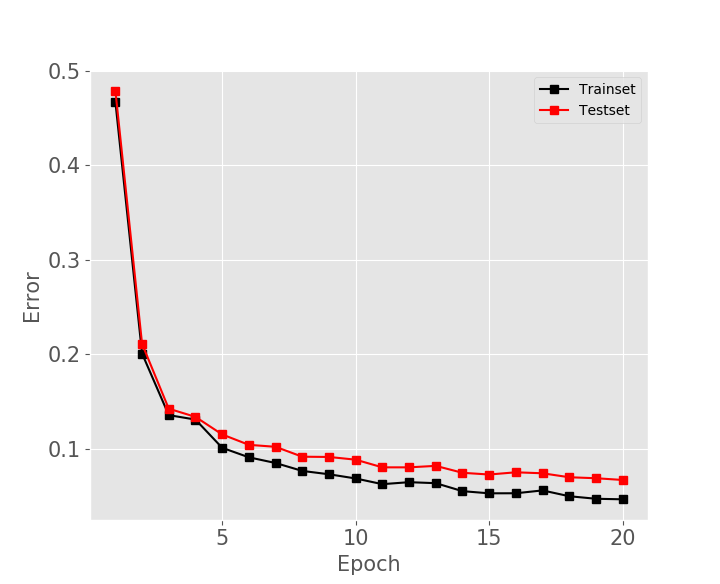
\includegraphics[width=.65\linewidth]{classification}
\end{center}
\end{center}

\begin{itemize}\compresslist
\item 93\% fucking beast
\end{itemize}

\begin{center}
%\includegraphics[width=.65\linewidth]{}
\end{center}


%------------------------------------------------

\begin{center}
\subsection*{TextGen and Classification}
\begin{center}
	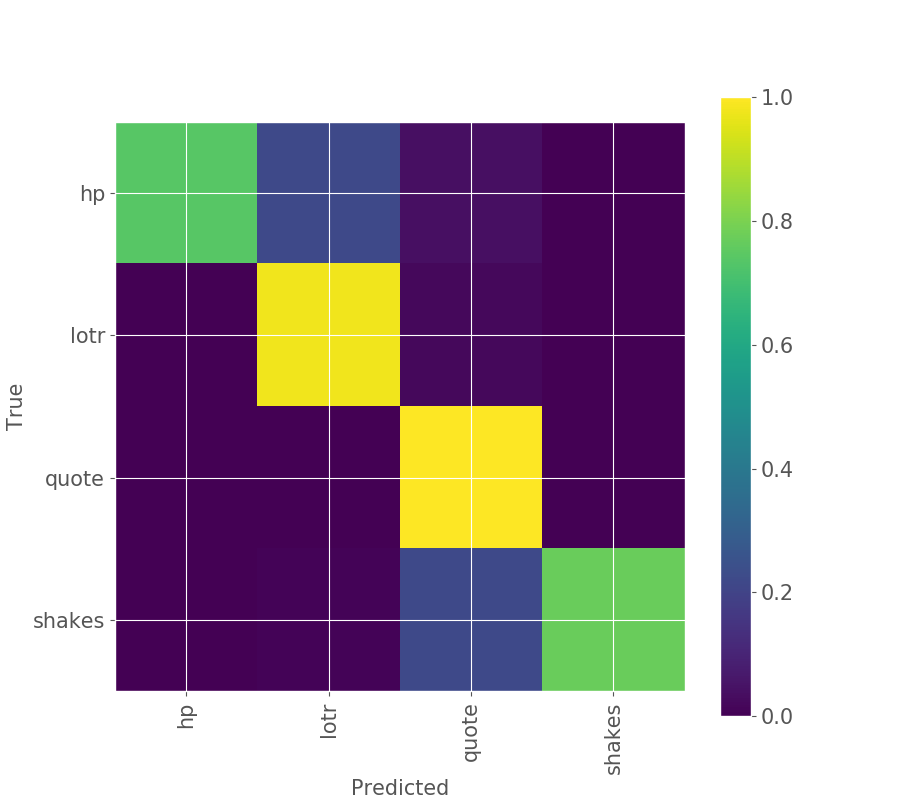
\includegraphics[width=.65\linewidth]{confusiontextgenwithpunc}
\end{center}
\end{center}
\begin{itemize}\compresslist
\item rocking this shit with 87\%
\end{itemize}

\end{multicols}

\vspace{-1 cm}
\begin{center}
\subsection*{Conclusion}
\end{center}

\begin{itemize}\compresslist
\item we love you simon
\item best project 100\%
\end{itemize}
% When there are two boxes, some whitespace may need to be added if the one on the right has more content
}

%----------------------------------------------------------------------------------------
%	REAL DATA 
%----------------------------------------------------------------------------------------

\headerbox{Blablabl}{name=CLSA,column=2,span=2,below=results, above=bottom}{
\vspace{0.25 cm}


\begin{multicols}{2}
\begin{itemize}\compresslist
\item \textbf{Comorbidity} : Any distinct additional clinical entity that has existed during the clinical course of a patient.
\item \textbf{CLSA database} : 50,000 patients and 58 \\comorbidity factors.
\item \textbf{Objective} : Profile the burden of comorbidity based on conditional dependences.
\end{itemize}

\vspace{-1 cm}
\begin{center}
%\includegraphics[width=1.3\linewidth]{}
\end{center}

\end{multicols}

\vspace{-1 cm}
\begin{center}
\textbf{Conclusion}
\end{center}

\begin{itemize}\compresslist
\item Highlight mechanisms of disease purely based on observational data.
\item Focus on few interesting associations which can then be specically tested in model organisms and clinical trials.
\end{itemize}


\vspace{0.3em} % When there are two boxes, some whitespace may need to be added if the one on the right has more content
}

%----------------------------------------------------------------------------------------
%	CONCLUSION 
%----------------------------------------------------------------------------------------

%\headerbox{Further Work}{name=conclusion,column=2,span=2,below=CLSA,above=bottom}{

%\begin{itemize}\compresslist
%\item Exploration and development of loss functions on unknown graph structure is a relevant idea.
%\end{itemize}

%\vspace{0.3em} % When there are two boxes, some whitespace may need to be added if the one on the right has more content
%}




\end{poster}

\end{document}